%%%%%%%%%%%%%%%%%%%%%%%%%%%%%%%%%%%%%%%%%
%
% (c) 2019 by Jennifer Laaser
%
% This work is licensed under the Creative Commons Attribution-NonCommercial-ShareAlike 4.0 International License. To view a copy of this license, visit http://creativecommons.org/licenses/by-nc-sa/4.0/ or send a letter to Creative Commons, PO Box 1866, Mountain View, CA 94042, USA.
%
% The current source for these materials is accessible on Github: https://github.com/jlaaser/pogil-polymers
%
%%%%%%%%%%%%%%%%%%%%%%%%%%%%%%%%%%%%%%%%%

\renewcommand{\figpath}{content/polymphys/solution-thermo/phase-diagrams/figs}
\renewcommand{\labelbase}{phase-diagrams}

\begin{activity}{Phase Diagrams of Polymer Solutions}

\begin{instructornotes}

	This activity introduces students to key concepts related to phase diagrams of polymer solutions.
	
	After completing this activity, students will be able to:
			\begin{enumerate}
				\item Sketch the phase diagram of a polymer solution that obeys Flory-Huggins theory
				\item Identify the critical point on a phase diagram and explain how its position changes with changes in chain length
				\item Identify the theta temperature of a polymer solution from information about its phase behavior
			\end{enumerate}
			
	\subsection*{Activity summary:}
	\begin{itemize}
		\item \textbf{Activity type:} Learning Cycle
		\item \textbf{Content goals:} See above %Phase diagrams of polymer solutions
		\item \textbf{Process goals:} %https://pogil.org/uploads/attachments/cj54b5yts006cklx4hh758htf-process-skills-official-pogil-list-2015-original.pdf
			\begin{itemize}
				\item Reading and interpreting graphs
				\item Extrapolating from given data
				\item Written and oral communication of reasoning
			\end{itemize}
		\item \textbf{Duration:} 60 minutes, including class discussion
		\item \textbf{Instructor preparation required:} none beyond knowledge of relevant content
		\item \textbf{Related textbook chapters:}
			\begin{itemize}
				\item \emph{Polymer Chemistry} (Hiemenz \& Lodge), 2nd ed.: sections 7.5.4 and 7.5.5, and parts of section 7.6
				\item \emph{Introduction to Polymers} (Young \& Lovell), 3rd ed.: not covered in detail
			\end{itemize}
	\end{itemize}

\end{instructornotes}

	%\textbf{Focus question:} Put a central question for the students to consider through this exercise here.


\begin{model}[From Free Energy Curves to Phase Diagrams]
\label{\labelbase:mdl:spinodalbinodal}

	Schematic free energy curves for solutions of polymers with the same degree of polymerization, $N$, but different values of $\chi$, are shown below:
	
	\centerline{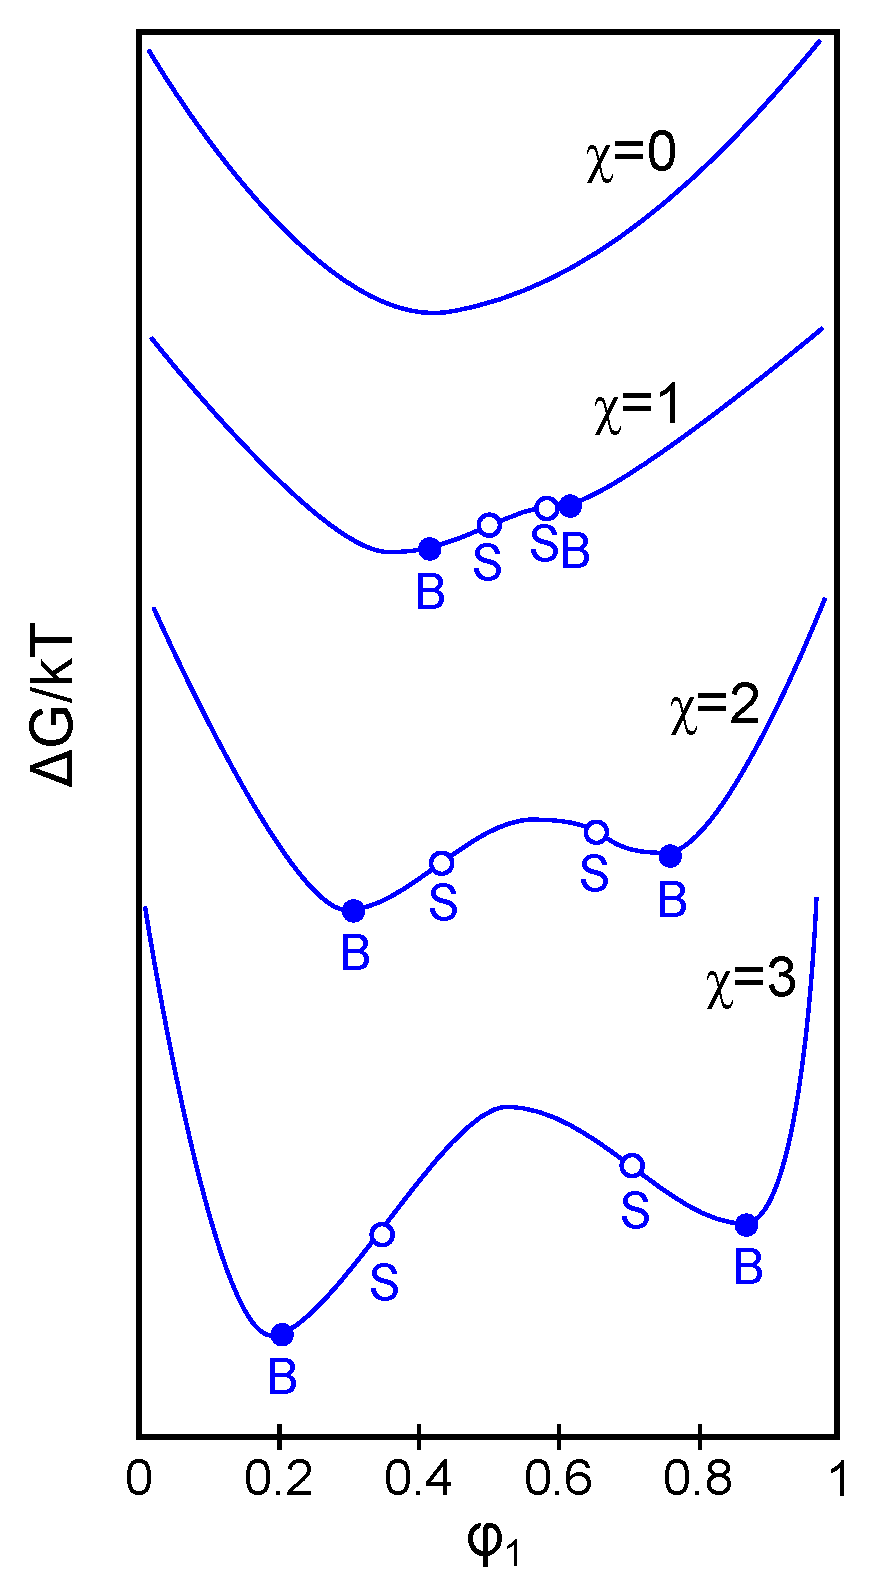
\includegraphics[width=0.4\textwidth]{\figpath/model1-varychi}}
	
	The spinodal (S) and binodal (B) points are marked on the plots where appropriate.
\end{model}

\begin{ctqs}

	\question For which value(s) of $\chi$ will the mixtures...
	
		\begin{enumerate}
			\item ... always form a homogeneous, single-phase solution?
				
				\begin{solution}[0.75in]{}
					0
				\end{solution}
			
			\item ... phase separate, for some values of $\phi_1$?
				\begin{solution}[0.75in]{}
					1, 2, 3
				\end{solution}
		\end{enumerate}
		
	\question Plot the locations of the spinodal and binodal points for each value of $\chi$ on the following axes.  When you have plotted all of the points, draw a smooth curve connecting all of the binodal points, and a second curve connecting all of the spinodal points.
	
		\begin{solution}[2in]{\centerline{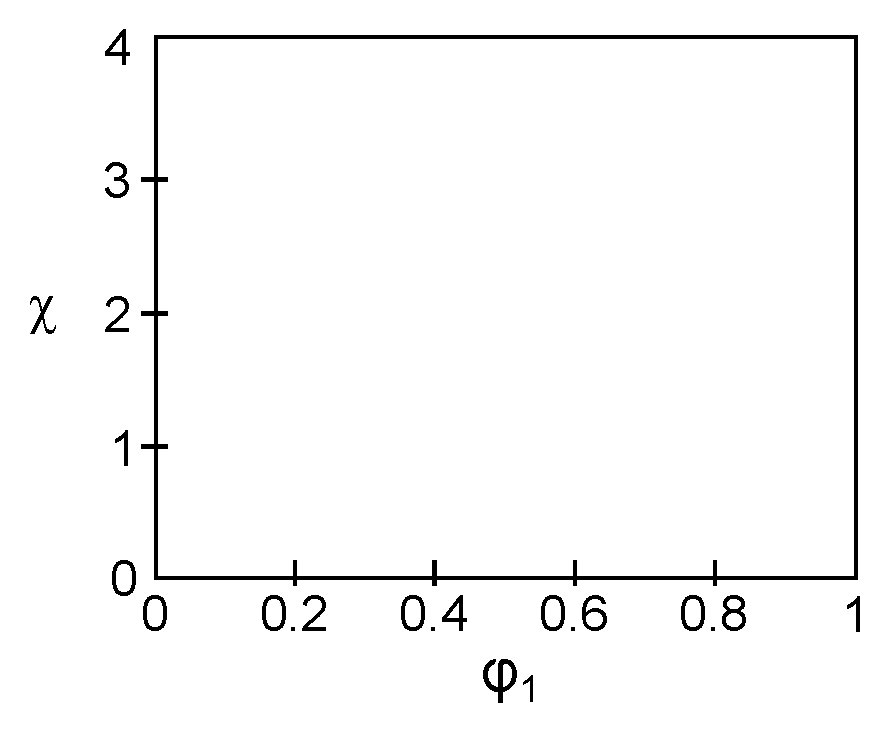
\includegraphics[width=0.45\textwidth]{\figpath/model1-phasediagramchi}}}
		\centerline{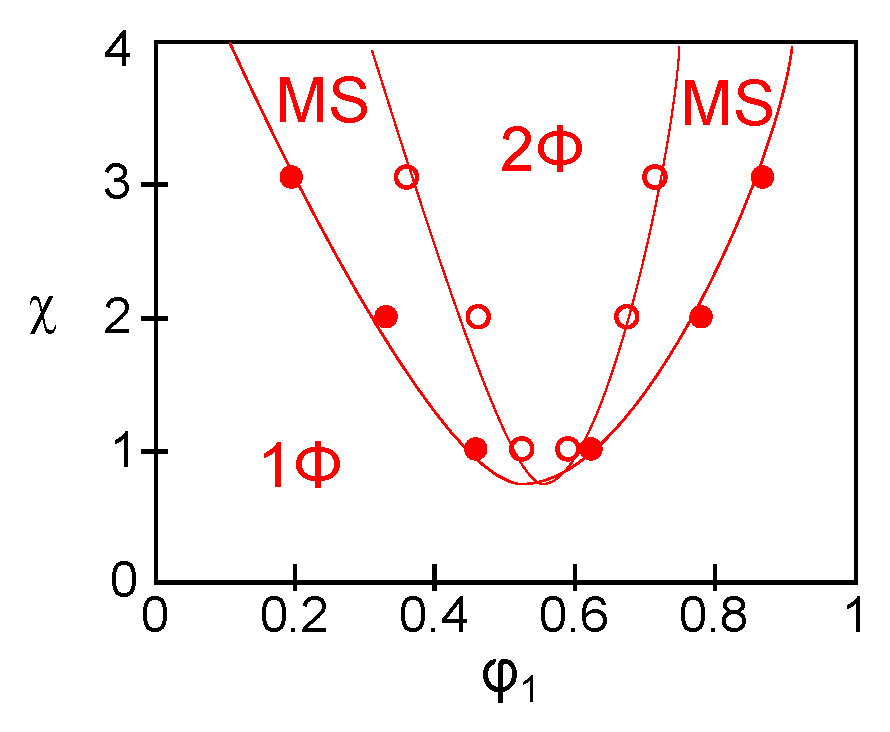
\includegraphics[width=0.45\textwidth]{\figpath/model1-phasediagramchi-answer}}
		\end{solution}
		
	\question On your plot, label the region in which you expect to always get a one-phase mixture as ``1$\Phi$'', the region in which you expect to always get a two-phase mixture as ``2$\Phi$'', and the region in which you expect to get a metastable one-phase mixture as ``MS''.
		
\end{ctqs}


\begin{infobox}
	For a given polymer/solvent pair, the interaction parameter, $\chi$, generally varies with temperature as
	\begin{equation*}
		\chi = \frac{\alpha}{T} + \beta
	\end{equation*}
\end{infobox}


\begin{ctqs}

	\question Re-plot your curves from the previous question with temperature on the y axis.  For the purposes of this problem, assume that this mixture has $\alpha=200$~K and $\beta=0$.
		\label{\labelbase:ctq:plotT}
	
		\begin{solution}[2in]{\centerline{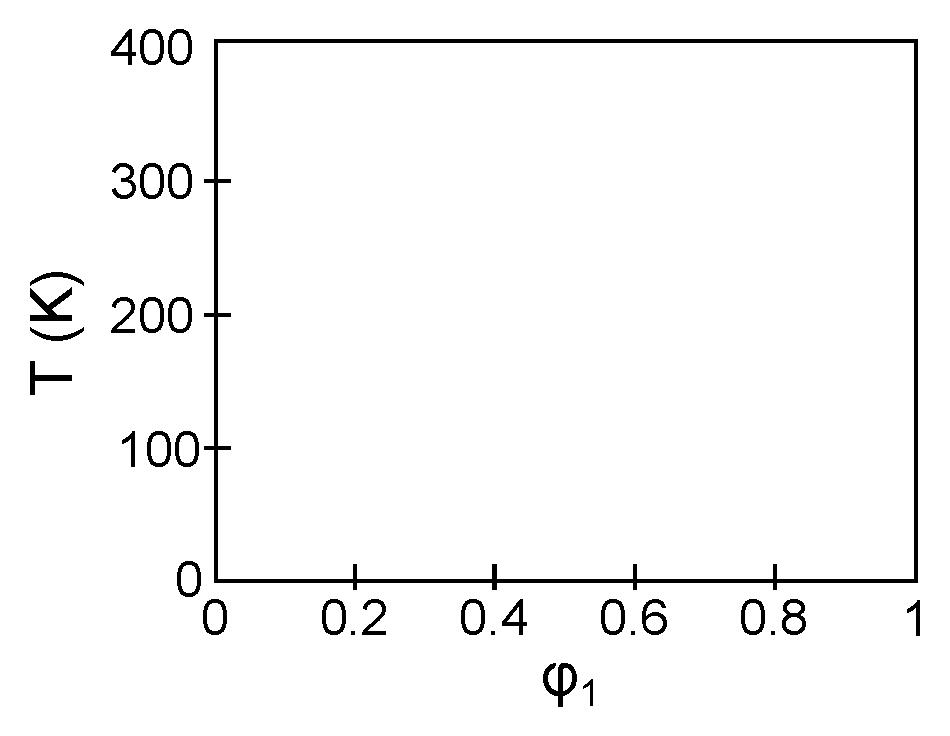
\includegraphics[width=0.5\textwidth]{\figpath/model1-phasediagramT}}}
		\centerline{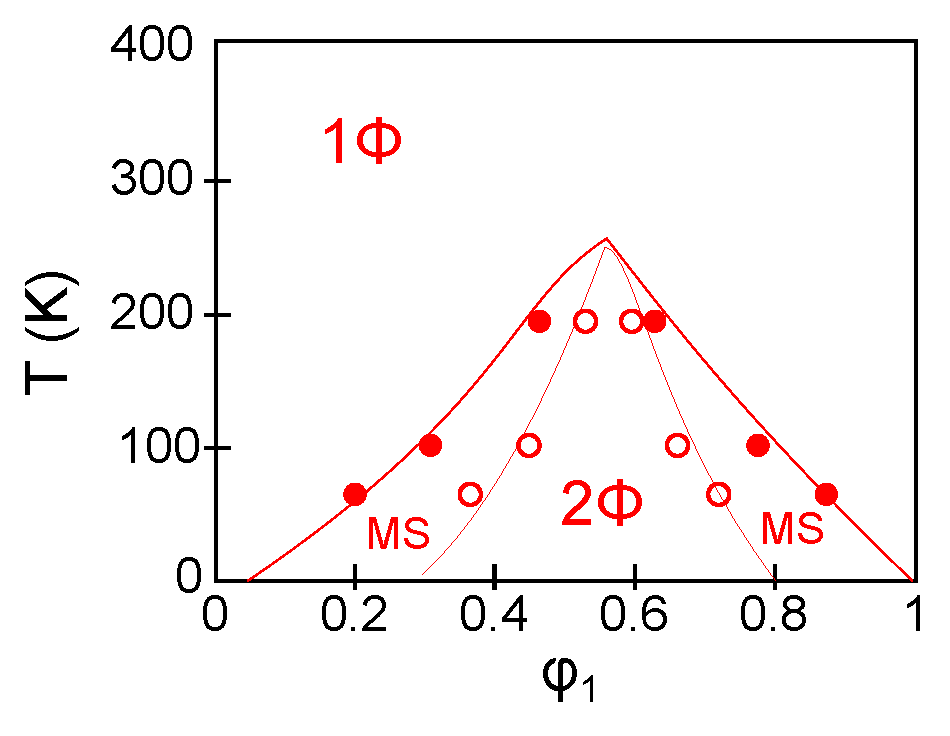
\includegraphics[width=0.5\textwidth]{\figpath/model1-phasediagramT-answer}}
		\end{solution}
		
	\question On your plot, label the region in which you expect to always get a single-phase mixture as ``1$\Phi$'', the region in which you expect to always get a two-phase mixture as ``2$\Phi$'', and the region in which you expect to get a metastable mixture as ``MS''.
		
		
\end{ctqs}


\begin{infobox}

	The \emph{critical temperature} of a polymer solution, $T_c$, is the temperature above which the mixture will \emph{always} form a homogeneous, single-phase solution.

\end{infobox}


\begin{ctqs}
	\question Estimate the critical temperature for the polymer whose phase diagram you drew in question \ref{\labelbase:ctq:plotT}.
	
		\begin{solution}[0.25in]{}
		
			Most students will guess something in the range of 250 to 300~K, but the exact number is not critical for this question.
		
		\end{solution}
		
\end{ctqs}



\begin{model}[Phase Diagrams of Polymer Solutions]
	\label{\labelbase:mdl:Ndependence}

	Spinodal curves calculated for a series of polymers with different degrees of polymerization $N$ are shown below:
	
	\centerline{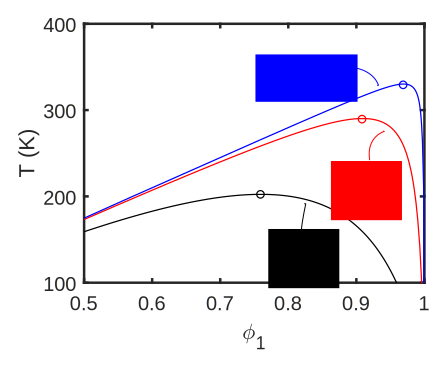
\includegraphics[width=0.5\textwidth]{\figpath/model2-spinodalN-edited}}
	
	The critical point for each curve is indicated with a circle ($\circ$).
	
\end{model}

\begin{ctqs}

	\question Estimate the critical temperature, $T_c$, and the composition at the critical point, $\phi_{1,c}$, for each value of $N$ shown in Model \ref{\labelbase:mdl:Ndependence}:
	
		\begin{center}
			\renewcommand{\arraystretch}{2.5}
			\begin{tabular}{|c|c|c|}
				\hline
				\textbf{N} & \hspace{0.6cm}$\phi_{1,c}$\hspace{0.6cm} & \hspace{0.75cm}$T_c$\hspace{0.75cm} \\\hline
				10 & \answer{0.76} & \answer{195 K} \\\hline
				100 & \answer{0.91} & \answer{290 K} \\\hline
				1000 & \answer{0.98} & \answer{320 K}\\\hline
			\end{tabular}
		\end{center}
		
	\question How do $\phi_{1,c}$ and $T_c$ change as $N$ increases?
	
		\begin{solution}[0.4in]{}
			$\phi_{1,c}$ and $T_c$ both increase as $N$ increases
		\end{solution}
	
	\question What do you expect to happen to the value of $\phi_{1,c}$ in the limit of infinitely long polymer chains ($N\to\infty$)?
	
		\begin{solution}[0.4in]{}
			It looks like $\phi_{1,c}$ will approach 1 as $N\to\infty$.
		\end{solution}
		
	\question What do you expect to happen to the value of $T_c$ in the limit of infinitely long polymer chains ($N\to\infty$)? \label{\labelbase:ctq:extrapTc}
	
		\begin{solution}[0.4in]{}
			In this case, it looks like $T_c$ will max out around 350 K.
			
			(If students get stuck, suggest they draw a line connecting the critical points and see where it passes through $\phi_{1,c}=1$.)
		\end{solution}

\end{ctqs}


\begin{infobox}
\label{\labelbase:infobox:critpt}
	
	The critical point occurs when the spinodal (and binodal) points converge.  Mathematically, the spinodal points occur when the second-derivative of the free energy is zero:
	\begin{equation*}
		\frac{d^2\Delta G}{d\phi_1^2} = 0
	\end{equation*}
	When the two spinodal points are on top of each other, the \emph{third} derivative of the free energy must also be zero; thus the critical point occurs when 
	\begin{equation*}
		\frac{d^3\Delta G}{d\phi_1^3} = 0
	\end{equation*}
	
	Applying these two conditions (see Exercise \ref{\labelbase:exc:critpt}), we find that the composition at the critical point is
	\begin{equation*}
		\phi_{1,c} = \frac{\sqrt{N}}{1+\sqrt{N}}
		\label{\labelbase:eqn:phi1c}
	\end{equation*}
	and the interaction parameter at the critical point is
	\begin{equation*}
		\chi_c = \frac{1}{2}\left(\frac{1}{N} + \frac{2}{\sqrt{N}} + 1\right)
		\label{\labelbase:eqn:chic}
	\end{equation*}
	
\end{infobox}



\begin{ctqs}
	
	\question What is the value of $\chi_c$ when the chains are only a single monomer long (i.e. when $N=1$)?
	
		\begin{solution}[0.75in]{}
			When $N=1$, $\chi_c = 2$
		\end{solution}
	
	\question What is the value of $\chi_c$ when the chains are infinitely long (i.e. when $N\to\infty$)?	
	
		\begin{solution}[0.75in]{}
			When $N\to\infty$, $\chi_c = \frac{1}{2}$.
		\end{solution}
	
	\question Based on your answers to the previous questions, critique or defend the following statement:
	
		\emph{``When $\chi > 0.5$, a polymer solution will always phase separate.'' }
	
		\begin{solution}[2.5in]{}
			This statement is \emph{not} correct.  Students may take one of two approaches when critiquing this statement:
			
			First, some students will give the intended reason, that when the chains are short, the critical value of $\chi$ is larger than $\frac{1}{2}$ and may be as large as 2.  So, for short chains, you can't guarantee that there will be phase separation until you reach $\chi = 2$.
			
			Second, some students will instead note that even when the value of $\chi$ is high enough that phase separation is likely, the problem did not tell us anything about whether the \emph{composition} is in the two-phase region of the phase diagram.  This is also a valid critique, if not the one intended by the question.
		\end{solution}

\end{ctqs}


\begin{infobox}
	
	The \emph{theta temperature} of a polymer solution is the temperature at which $\chi=0.5$.
	
\end{infobox}


\begin{ctqs}

	\question Explain, in 2-3 complete sentences, why the theta temperature can also be described as the temperature above which all polymer chains are soluble, regardless of their molecular weight.
	
		\begin{solution}[2.25in]{}
			The theta temperature occurs at $\chi_c =0.5$, which, as we learned above, is the value of $\chi_c$ in the limit that $N\to\infty$.  In other words, the theta temperature is the same as the critical temperature in the limit that the degree of polymerization (and thus molecular weight) goes to infinity, and above this temperature all polymer chains will be soluble no matter what their molecular weight.
		\end{solution}
	
	\question Propose a method that you could use to find the theta temperature of a polymer/solvent mixture from phase diagrams such as those shown in Model \ref{\labelbase:mdl:Ndependence}.
	
		\begin{solution}[1.25in]{}
			Draw a line connecting all of the critical points, and look at the temperature at the point where this line crosses $\phi_{1,c} =1$
			
			\emph{Note: strictly speaking, the curve connecting the critical points is quadratic in $\phi_1$, not linear.  However, for values of $N$ greater than about 10, a line serves as a reasonable approximation.}
		\end{solution} 

	\question Using your method, estimate the theta temperature for the polymer shown in Model \ref{\labelbase:mdl:Ndependence}.
	
		\begin{solution}[0.5in]{}
			350 K (same as the answer to CTQ \ref{\labelbase:ctq:extrapTc})
		\end{solution} 

\end{ctqs}



\begin{exercises}

	\exercise Derive the expressions for $\phi_{1,c}$ and $\chi_c$ given in the activity by doing the following:
		\label{\labelbase:exc:critpt}
	
		\begin{enumerate}
	
			\item First, show that the third derivative of the Flory-Huggins expression for the free energy of a polymer solution is
				\begin{equation*}
					\frac{d^3\Delta G}{d\phi_1^3} = \frac{-1}{\phi_1^2} + \frac{1}{N}\frac{1}{(1-\phi_1)^2}
				\end{equation*}
		
				Then set this expression equal to zero and solve for $\phi_{1,c}$, the composition at the critical point.
			
				\begin{solution}{}
					The Flory-Huggins expression for the free energy of a polymer solution is 
					\begin{equation*}
						\frac{\Delta G_{mix}}{k_B T} = \phi_1\phi_2\chi + \phi_1\ln\phi_1 + \frac{\phi_2}{N}\ln\phi_2
					\end{equation*}
					Noting that $\phi_2 = 1-\phi_1$, this expression can alternately be written
					\begin{equation*}
						\frac{\Delta G_{mix}}{k_B T} = \phi_1(1-\phi_1)\chi + \phi_1\ln\phi_1 + \frac{(1-\phi_1)}{N}\ln(1-\phi_1)
					\end{equation*}
					Taking the first derivative, we obtain
					\begin{align*}
						\frac{ d\Delta G}{d\phi_1} &= \chi(1-2\phi_1) + \left(\phi_1\frac{1}{\phi_1} + \ln\phi_1\right) + \frac{1}{N}\left((1-\phi_1)\frac{-1}{1-\phi_1} - \ln(1-\phi_1)\right)\\
							&= \chi(1-2\phi_1) + (1 + \ln\phi_1) - \frac{1}{N}\left(1 + \ln(1-\phi_1)\right)
					\end{align*}
					The second derivative is then
					\begin{align*}
						\frac{d^2\Delta G}{d\phi_1^2} &= \chi(-2) + \left(0 + \frac{1}{\phi_1}\right)-\frac{1}{N}\left(0 + \frac{-1}{1-\phi_1}\right)\\
							&= -2\chi +\frac{1}{\phi_1} + \frac{1}{N}\frac{1}{1-\phi_1}
					\end{align*}
					\end{solution}  % need to allow a page break in here!
					\begin{solution}{}
					Finally, the third derivative is
					\begin{align*}
					\frac{d^3\Delta G}{d\phi_1^3} = \frac{-1}{\phi_1^2} + \frac{1}{N}\frac{1}{(1-\phi_1)^2}
					\end{align*}
					as desired.
					
					Setting this expression equal to zero and rearranging, we obtain
					\begin{align*}
						\frac{1}{N}\frac{1}{(1-\phi_1)^2} &= \frac{1}{\phi_1^2}\\
						\frac{1}{\sqrt{N}}\frac{1}{1-\phi_1} &= \frac{1}{\phi_1}\\
						\sqrt{N}(1-\phi_1) &= \phi_1\\
						\phi_1(1+\sqrt{N}) &= \sqrt{N}\\
						\phi_{1,c} &= \frac{\sqrt{N}}{1+\sqrt{N}}
					\end{align*}
					as desired.
				\end{solution}
				
		
			\item Second, show that the second derivative of the Flory-Huggins expression for the free energy of a polymer solution is
	
				\begin{equation*}
					\frac{d^2\Delta G}{d\phi_1^2} = -2\chi + \frac{1}{\phi_1} + \frac{1}{N}\frac{1}{1-\phi_1}
				\end{equation*}
		
				Set this expression equal to zero and solve for $\chi$ in terms of $\phi_1$.
			
				\begin{solution}{}
					The above expression for $\frac{d^2\Delta G}{d\phi_1^2}$ was obtained in the previous part of the problem.  Setting it equal to 0 and solving for $\chi$, we obtain
					\begin{align*}
						0 &= -2\chi + \frac{1}{\phi_1} + \frac{1}{N}\frac{1}{1-\phi_1}\\
						2\chi &= \frac{1}{\phi_1} + \frac{1}{N}\frac{1}{1-\phi_1}\\
						\chi &= \frac{1}{2}\left(\frac{1}{\phi_1} + \frac{1}{N}\frac{1}{1-\phi_1}\right)
					\end{align*}
				\end{solution}
				
				
			\item Finally, substitute in your expression for $\phi_{1,c}$ to find $\chi_c$, the interaction parameter at the critical point, and verify that it is consistent with the equation given on page \pageref{\labelbase:infobox:critpt}.
			
				\begin{solution}{}
					Combining our results from the previous two parts, we obtain
					\begin{align*}
						\chi_c &= \frac{1}{2}\left(\frac{1}{\frac{\sqrt{N}}{1+\sqrt{N}}} + \frac{1}{N}\frac{1}{1-\frac{\sqrt{N}}{1+\sqrt{N}}}\right)\\
							&= \frac{1}{2}\left(\frac{1+\sqrt{N}}{\sqrt{N}} + \frac{1}{N}\frac{1+\sqrt{N}}{1+\sqrt{N}-\sqrt{N}}\right)\\
							&= \frac{1}{2}\left(\frac{1}{\sqrt{N}} + 1 +\frac{1}{N}(1+\sqrt{N})\right)\\
							&= \frac{1}{2}\left(\frac{1}{\sqrt{N}} + 1 + \frac{1}{N} + \frac{1}{\sqrt{N}}\right)\\
							&= \frac{1}{2}\left(\frac{1}{N} + \frac{2}{\sqrt{N}}+1\right)
					\end{align*}
					as desired.
				\end{solution}
				
				
		\end{enumerate}
		
	\exercise Do the following for a polymer solution for which $\chi = \alpha/T$:
		
		\begin{enumerate}
			\item Find an expression for the critical temperature, $T_c$, in terms of the degree of polymerization, $N$.
			
				\begin{solution}{}
					Using
					\begin{equation*}
						\chi = \frac{\alpha}{T}
					\end{equation*}
					and
					\begin{equation*}
						\chi_c = \frac{1}{2}\left(\frac{1}{N} + \frac{2}{\sqrt{N}} + 1\right)
					\end{equation*}
					we find that
					\begin{equation*}
						T_c = \frac{\alpha}{\chi_c} = \frac{\alpha}{\frac{1}{2}\left(\frac{1}{N} + \frac{2}{\sqrt{N}} + 1\right)} = \frac{2\alpha N}{1 + 2\sqrt{N} + N}
					\end{equation*}
				\end{solution}
				
			\item Find an expression for the theta temperature  in terms of $\alpha$.
			
				\begin{solution}{}
					To answer this question, we need to take the limit of the previous expression as $N\to\infty$:
					\begin{equation*}
						T_\theta = \lim_{N\to\infty} \frac{\alpha}{\frac{1}{2}\left(\frac{1}{N} + \frac{2}{\sqrt{N}} + 1\right)} = \frac{\alpha}{\frac{1}{2}} = 2\alpha
					\end{equation*}
					Alternatively, we can just recognize that at the theta temperature, $\chi_c = \frac{1}{2}$ and skip directly to $T_\theta = \frac{\alpha}{1/2} = 2\alpha$.
				\end{solution}
				
		\end{enumerate}
		
	\exercise For the polymer solution whose spinodal curve is shown below,
	
		\centerline{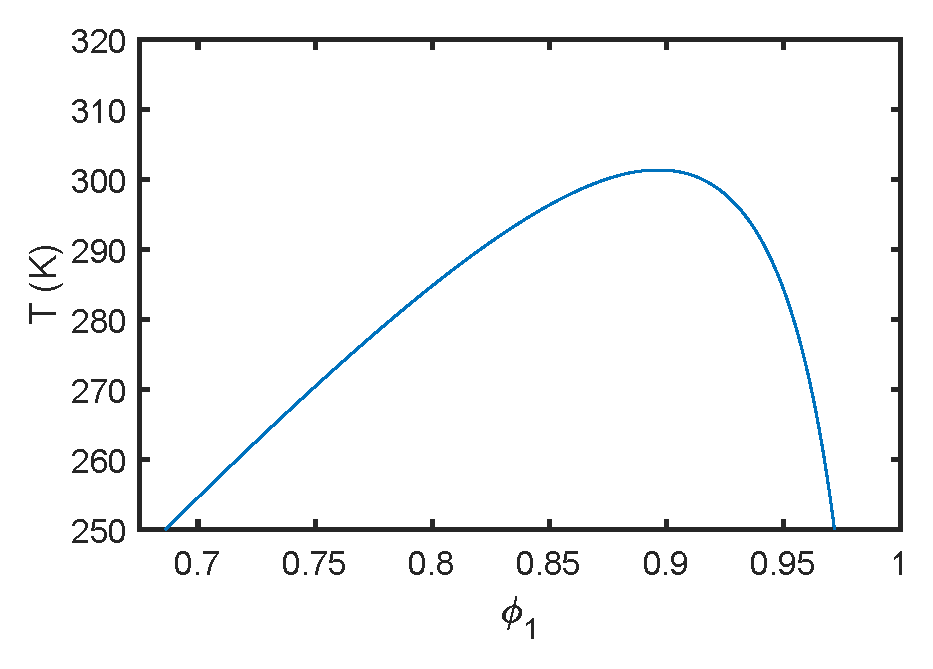
\includegraphics[width=0.5\textwidth]{\figpath/exercise-samplespinodal}}
	
		\begin{enumerate}
			\item Estimate the degree of polymerization of the polymer.
				
				\emph{Hint: start by finding the composition at the critical point, $\phi_{1,c}$.}
			
				\begin{solution}{}
					%Correct answer: 75
					The composition at the critical point, $\phi_{1,c}$, appears to be approximately 0.90. From the information box on page \pageref{\labelbase:eqn:phi1c}, we know that
					\begin{equation*}
						\phi_{1,c} = \frac{\sqrt{N}}{1+\sqrt{N}}
					\end{equation*}
					Solving for $N$, we obtain
					\begin{equation*}
						N = \left(\frac{\phi_{1,c}}{1-\phi_{1,c}}\right)^2 = \left(\frac{0.9}{0.1}\right)^2 = 81
					\end{equation*}
					Thus the degree of polymerization of the polymer is approximately 80.
				\end{solution}
				
			\item Estimate the interaction parameter, $\chi$, for this polymer mixture at the critical point.
			
				\begin{solution}{}
					The interaction parameter at the critical point, again from the information box on page \pageref{\labelbase:eqn:phi1c}, is
					\begin{equation*}
						\chi_c = \frac{1}{2}\left(\frac{1}{N} + \frac{2}{\sqrt{N}} + 1\right)
					\end{equation*}
					Plugging in $N=81$, we obtain
					\begin{equation*}
						\chi_c = \frac{1}{2}\left(\frac{1}{81} + \frac{2}{9} +1\right) = 0.62
					\end{equation*}
				\end{solution}
				
			
			\item Finally, estimate the theta temperature for this polymer system, assuming that $\chi$ obeys the relationship $\chi = \frac{\alpha}{T}$.
			
				\begin{solution}{}
					%Correct answer: 375 K
					
					The critical point on the plot appears to occur at a temperature of about 300~K.  Given that
					\begin{equation*}
						\chi = \frac{\alpha}{T}
					\end{equation*}
					we obtain
					\begin{equation*}
						\alpha = \chi_c T_c = (0.62)(300\text{ K}) = 186\text{ K}
					\end{equation*}
					Because the theta point occurs when $\chi_c = 0.5$, we find
					\begin{equation*}
						T_\theta = \frac{\alpha}{0.5} = \frac{186\text{ K}}{0.5} = 372\text{ K}
					\end{equation*}
					Thus the theta temperature of this polymer is approximately 370 K.
					
					\emph{Note: the phase diagram in the question was actually calculated $N=75$ and $T_\theta = 375\text{ K}$, so this approach got pretty close!}
					
					%\emph{Note \#2: this question asked students to find the theta temperature, but could equivalently have asked them to find the temperature above which all polymer chains will be soluble regardless of molecular weight.}
				\end{solution}
				
			
		\end{enumerate}
		
	\exercise What do you expect would happen if you prepared a polymer solution at a very high temperature and then rapidly cooled the mixture to a temperature below its critical point?  Explain your reasoning in 2-3 complete sentences.
			
				\begin{solution}{}
					Depending on the composition of the mixture, some or all of the polymer might precipitate out of solution as the temperature is changed such that you move from the one-phase region of the phase diagram into the two-phase region of the diagram.
					
					Note that if the polymer has a broad molecular weight distribution, the higher molecular weight fraction will crash out of solution first, while some of the lower molecular weight polymers may remain in solution, depending on the final temperature.
				\end{solution}
				
		
\end{exercises}
	
\end{activity}